\documentclass[11pt,a4paper]{article}

\usepackage[utf8]{inputenc}
\usepackage[T1]{fontenc}
\usepackage{lmodern}
\usepackage[margin=0.82in]{geometry}
\usepackage[table]{xcolor}
\usepackage{array}
\usepackage{tabularx}
\usepackage{booktabs}
\usepackage{enumitem}
\usepackage{titlesec}
\usepackage{fancyhdr}
\usepackage{lastpage}
\usepackage{hyperref}
\usepackage{tikz}

\definecolor{TextInk}{HTML}{233142}
\definecolor{HeadingBlue}{HTML}{1D3557}
\definecolor{AccentTeal}{HTML}{2A7F92}
\definecolor{AccentGold}{HTML}{C58B4E}
\definecolor{RuleGray}{HTML}{D6E0E5}
\definecolor{TableStripe}{HTML}{F3F8FA}
\definecolor{SoftTint}{HTML}{F7F4EE}
\definecolor{SoftBlue}{HTML}{EEF6F8}
\definecolor{SoftGreen}{HTML}{EEF7F0}
\definecolor{SoftRed}{HTML}{FBF0EF}

\hypersetup{
  colorlinks=true,
  linkcolor=HeadingBlue,
  urlcolor=AccentTeal,
  pdftitle={IB Geography SL Study Pack - 2026-04-26},
  pdfauthor={IB Geography SL Preparation}
}

\color{TextInk}
\setlength{\parskip}{0.52em}
\setlength{\parindent}{0pt}
\setlength{\tabcolsep}{6pt}
\renewcommand{\arraystretch}{1.22}
\setlist[itemize]{leftmargin=1.35em,itemsep=3pt,topsep=4pt}
\setlist[enumerate]{leftmargin=1.5em,itemsep=3pt,topsep=4pt}

\newcolumntype{Y}{>{\raggedright\arraybackslash}X}
\newcolumntype{L}[1]{>{\raggedright\arraybackslash}p{#1}}

\titleformat{\section}
  {\normalfont\huge\sffamily\bfseries\color{HeadingBlue}}
  {}{0pt}{}
  [\vspace{0.15em}{\color{AccentGold}\titlerule[1pt]}]

\titleformat{\subsection}
  {\normalfont\Large\sffamily\bfseries\color{AccentTeal}}
  {}{0pt}{}

\titleformat{\subsubsection}
  {\normalfont\large\sffamily\bfseries\color{HeadingBlue}}
  {}{0pt}{}

\titlespacing*{\section}{0pt}{1.4em}{0.65em}
\titlespacing*{\subsection}{0pt}{1.0em}{0.35em}
\titlespacing*{\subsubsection}{0pt}{0.8em}{0.25em}

\pagestyle{fancy}
\setlength{\headheight}{14pt}
\fancyhf{}
\fancyhead[L]{\sffamily\color{AccentTeal}Sun 2026-04-26}
\fancyhead[R]{\sffamily\color{HeadingBlue}IB Geography SL}
\fancyfoot[C]{\sffamily\color{HeadingBlue}\thepage\ of \pageref{LastPage}}
\renewcommand{\headrulewidth}{0.4pt}
\renewcommand{\footrulewidth}{0pt}

\newcommand{\term}[1]{\textcolor{HeadingBlue}{\textbf{#1}}}
\newcommand{\exam}[1]{\textcolor{AccentTeal}{\textbf{#1}}}
\newcommand{\boxnote}[3]{%
\noindent\colorbox{#1}{%
  \begin{minipage}{0.965\textwidth}
  \sffamily
  \textbf{\textcolor{HeadingBlue}{#2}} #3
  \end{minipage}
}}

\begin{document}

\begin{center}
  {\sffamily\bfseries\color{HeadingBlue}\LARGE IB Geography SL Study Pack}\\[0.25em]
  {\sffamily\bfseries\color{AccentTeal}\Large Sunday 2026-04-26}\\[0.35em]
  {\sffamily\color{TextInk}Food And Health Depth: Recall, Timed Practice, Marking, And Case-Study Drill}
\end{center}

\vspace{0.5em}

\boxnote{SoftBlue}{How this pack follows the plan.}{The April 26 schedule is a
weekend \term{90 minute} session: \term{30 minutes} closed-book recall of
\term{Food and health} subtopics, food systems, disease spread, and
stakeholders; \term{30 minutes} of Paper 1 structured-question style practice;
\term{20 minutes} to mark and log errors; and \term{10 minutes} to drill
case-study names and one evaluative point for each. This pack is designed for
direct PDF conversion with the same textbook-style color scheme as the April 24
and April 25 materials.}

\section{Today's Target}

By the end of this session, you should be able to:

\begin{itemize}
  \item recall the four main Food and health subtopic clusters without notes
  \item explain how a food system links production, processing, distribution,
  consumption, and waste
  \item distinguish \term{food security}, \term{malnutrition},
  \term{undernutrition}, and \term{overnutrition}
  \item explain how disease spreads through environmental, social, economic,
  and political factors
  \item identify stakeholders in food and health and evaluate who benefits or
  loses from their actions
  \item use the studied case-study anchor \term{TNCs in Brazil (Nestle)} with a
  clear evaluative point
\end{itemize}

\subsection{90-Minute Session Map}

\rowcolors{2}{TableStripe}{white}
\begin{tabularx}{\textwidth}{L{0.16\textwidth}Y L{0.24\textwidth}}
\toprule
\textbf{Time} & \textbf{Task} & \textbf{Output} \\
\midrule
0--30 min & Closed-book recall of Food and health subtopics, food systems,
disease spread, and stakeholders & One completed recall map \\
30--60 min & Timed structured-question practice & One full practice response \\
60--80 min & Self-mark, compare with the guide, and write an error log & Three
fixes to carry forward \\
80--90 min & Drill case-study names and one evaluative point for each & At
least four precise case-study entries checked \\
\bottomrule
\end{tabularx}
\rowcolors{2}{}{}

\section{30-Minute Recall Block}

\subsection{The Four-Cluster Map}

Before reading further, shut the pack and write the four Food and health
clusters from memory. Then reopen and check against this list:

\begin{enumerate}
  \item \term{Measuring food and health}
  \item \term{Food systems and the spread of diseases}
  \item \term{Stakeholders in food and health}
  \item \term{Future health, food security, and sustainability}
\end{enumerate}

These clusters are your sorting system. If a question asks about indicators,
calorie intake, life expectancy, infant mortality, obesity, undernutrition, or
access to healthcare, start with \term{measuring food and health}. If it asks
about production, trade, processing, retail, diets, waste, water-borne disease,
vector-borne disease, or diffusion, start with \term{food systems and disease
spread}. If it asks about TNCs, governments, NGOs, farmers, consumers, or
international organizations, start with \term{stakeholders}. If it asks about
food security, sustainable farming, changing diets, climate stress, or future
health risks, start with \term{future sustainability}. Key syllabus words that
belong in this option include \term{subsistence farming},
\term{commercial farming}, \term{agro-industrial farming}, \term{food miles},
\term{nutrition transition}, \term{disease diffusion}, and the
\term{water-energy-food nexus}.

\subsection{Keyword Warm-Up}

Use these terms during the 30-minute recall block. The final 10 minutes today
should stay focused on case-study names and evaluative points.

\rowcolors{2}{TableStripe}{white}
\begin{tabularx}{\textwidth}{L{0.28\textwidth}Y}
\toprule
\textbf{Term} & \textbf{Clean definition} \\
\midrule
Food security & Reliable physical, social, and economic access to sufficient,
safe, nutritious food for an active and healthy life. \\
Food system & The full chain of actors and processes involved in producing,
processing, distributing, consuming, and disposing of food. \\
Malnutrition & Poor nutrition caused by too little, too much, or imbalanced
intake of energy or nutrients. \\
Undernutrition & Insufficient intake or absorption of food energy, protein, or
nutrients. \\
Overnutrition & Excessive food energy or nutrient intake, often linked with
obesity and diet-related disease. \\
Nutrition transition & A shift in diet and health patterns, often from
traditional diets and infectious disease burdens toward processed foods,
obesity, and non-communicable disease. \\
Famine & Extreme food shortage causing widespread hunger, malnutrition, and
increased mortality. \\
Morbidity & Illness or disease within a population. \\
Mortality & Death within a population. \\
Communicable disease & A disease that can be transmitted between people or via
vectors, water, food, or other pathways. \\
Non-communicable disease & A disease that is not directly passed from person
to person, such as diabetes or heart disease. \\
Vector-borne disease & Disease transmitted by a living carrier such as a
mosquito. \\
Water-borne disease & Disease transmitted through contaminated water. \\
Diffusion & The spread of a disease, idea, product, or practice through space
and time. \\
Stakeholder & A person, group, company, government, or organization with an
interest in an issue. \\
TNC & A transnational corporation operating in more than one country. \\
Subsistence farming & Farming mainly to feed the farmer's household or local
community. \\
Commercial farming & Farming mainly to sell output for profit. \\
Agro-industrial farming & Large-scale, capital-intensive farming linked to
processing, technology, supply chains, and markets. \\
Food miles & The distance food travels from production to consumption. \\
Water-energy-food nexus & The interdependence between water supply, energy
production, and food production. \\
\bottomrule
\end{tabularx}
\rowcolors{2}{}{}

\subsection{Food And Health Measurement}

IB answers get stronger when they use indicators carefully. One indicator is
rarely enough. Combine food indicators with health indicators, then evaluate
what each one hides.

\rowcolors{2}{TableStripe}{white}
\begin{tabularx}{\textwidth}{L{0.23\textwidth}Y Y}
\toprule
\textbf{Indicator} & \textbf{What it can show} & \textbf{Limitation to remember} \\
\midrule
Daily calorie intake & Broad access to food energy & It does not show
micronutrient quality, distribution within households, or diet-related disease
risk \\
Undernourishment or child stunting & Long-term lack of enough food or nutrients
& It may hide short-term shocks or regional differences inside a country \\
Obesity rate & Overnutrition, processed-food diets, sedentary lifestyles, and
nutrition transition & It does not automatically mean everyone has equal food
choice or healthcare access \\
Life expectancy & Overall health, healthcare access, sanitation, nutrition, and
security & It is an average and can hide inequality by gender, income, region,
or ethnicity \\
Infant mortality rate & Maternal health, nutrition, clean water, sanitation,
and healthcare quality & It does not explain the exact cause without more
evidence \\
Morbidity or disease incidence & Burden of disease in a population & It depends
on testing, diagnosis, and reporting capacity \\
\bottomrule
\end{tabularx}
\rowcolors{2}{}{}

\boxnote{SoftTint}{Measurement-writing rule.}{A strong answer says:
\term{indicator} $\rightarrow$ \term{pattern} $\rightarrow$ \term{cause}
$\rightarrow$ \term{limitation}. Avoid treating one statistic as the whole
truth.}

\subsection{Food Systems}

A \term{food system} includes all the activities and actors involved in feeding
people. It includes inputs, farming, processing, storage, transport, retail,
consumption, waste, and policy. Food systems affect health because they shape
availability, access, price, diet quality, contamination risk, and long-term
sustainability.

\begin{center}
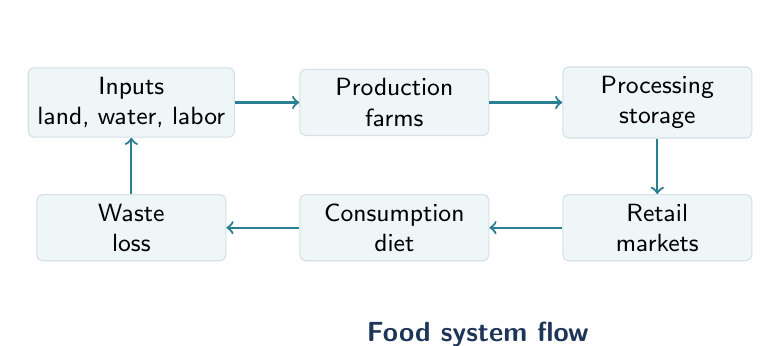
\begin{tikzpicture}[node distance=1.34cm, every node/.style={font=\sffamily\small}]
  \tikzstyle{stage}=[rectangle, rounded corners=2pt, draw=RuleGray, fill=SoftBlue,
  minimum width=2.4cm, minimum height=0.75cm, align=center]
  \node[stage] (inputs) {Inputs\\land, water, labor};
  \node[stage, right of=inputs, xshift=2.0cm] (production) {Production\\farms};
  \node[stage, right of=production, xshift=2.0cm] (processing) {Processing\\storage};
  \node[stage, below of=processing, yshift=-0.25cm] (retail) {Retail\\markets};
  \node[stage, left of=retail, xshift=-2.0cm] (consumption) {Consumption\\diet};
  \node[stage, left of=consumption, xshift=-2.0cm] (waste) {Waste\\loss};
  \draw[->, thick, color=AccentTeal] (inputs) -- (production);
  \draw[->, thick, color=AccentTeal] (production) -- (processing);
  \draw[->, thick, color=AccentTeal] (processing) -- (retail);
  \draw[->, thick, color=AccentTeal] (retail) -- (consumption);
  \draw[->, thick, color=AccentTeal] (consumption) -- (waste);
  \draw[->, thick, color=AccentTeal] (waste) -- (inputs);
  \node[font=\sffamily\bfseries\color{HeadingBlue}] at (4.4,-2.95) {Food system flow};
\end{tikzpicture}
\end{center}

\rowcolors{2}{TableStripe}{white}
\begin{tabularx}{\textwidth}{L{0.2\textwidth}Y Y}
\toprule
\textbf{Food-system factor} & \textbf{Health link} & \textbf{Evaluation angle} \\
\midrule
Agricultural production & Affects food availability, rural income, pesticide
exposure, and environmental quality & High output can improve supply but may
increase water use, soil stress, or chemical exposure \\
Processing and packaging & Can improve storage and reduce spoilage, but can
also increase sugar, salt, fat, and ultra-processed diets & Ask whether
convenience and profit align with long-term health \\
Transport and trade & Moves food from surplus to deficit regions and expands
choice & Dependence on imports can raise vulnerability to price shocks and
supply disruption \\
Retail and marketing & Shapes what consumers see, desire, and can afford &
Advertising and pricing may push less healthy products more strongly than
fresh foods \\
Waste and loss & Reduces the food actually available for consumption & Waste
reveals inefficiency even where production is high \\
\bottomrule
\end{tabularx}
\rowcolors{2}{}{}

\subsection{Disease Spread}

For disease spread, avoid one-cause answers. Disease patterns usually reflect
interaction between the pathogen, people, environment, mobility, healthcare,
and governance.

\rowcolors{2}{TableStripe}{white}
\begin{tabularx}{\textwidth}{L{0.19\textwidth}Y Y}
\toprule
\textbf{Disease factor} & \textbf{Examples} & \textbf{How to explain it} \\
\midrule
Environmental conditions & Water quality, climate, drainage, standing water,
housing density & Conditions can support pathogens, vectors, contamination, or
rapid person-to-person spread \\
Human movement & Migration, commuting, tourism, trade, conflict displacement &
Movement connects places and can accelerate diffusion across scales \\
Socio-economic inequality & Poverty, overcrowding, poor sanitation, weak food
storage, limited healthcare & Inequality affects exposure, vulnerability, and
ability to recover \\
Health systems & Clinics, vaccination, testing, public health messaging,
medicine access & Strong systems can reduce spread and mortality; weak systems
allow outbreaks to grow \\
Governance and trust & Regulation, emergency response, education, data
quality, public confidence & Policies work better when people can understand,
afford, and trust them \\
\bottomrule
\end{tabularx}
\rowcolors{2}{}{}

\boxnote{SoftBlue}{Disease-writing rule.}{Use the chain:
\term{condition} $\rightarrow$ \term{transmission route} $\rightarrow$
\term{vulnerable group} $\rightarrow$ \term{response}. If you have a named
disease case from class, use that place first.}

\subsection{Stakeholders In Food And Health}

Stakeholders are people or organizations with an interest in the issue. The
same stakeholder can create benefits and costs, so evaluation is essential.

\rowcolors{2}{TableStripe}{white}
\begin{tabularx}{\textwidth}{L{0.22\textwidth}Y Y}
\toprule
\textbf{Stakeholder} & \textbf{Possible role} & \textbf{Evaluation question} \\
\midrule
Farmers and fishers & Produce food, manage land or water, respond to prices
and climate risk & Are they gaining stable livelihoods or carrying most of the
risk? \\
TNCs & Invest in production, processing, retail, marketing, supply chains, and
jobs & Do they improve access and employment, or encourage unhealthy diets and
dependence? \\
Governments & Regulate food safety, healthcare, trade, school meals, subsidies,
and public health & Are policies reaching vulnerable groups or mainly helping
powerful actors? \\
NGOs and charities & Provide emergency food, health education, clinics, or
community support & Are they solving structural causes or only treating
symptoms? \\
Consumers and households & Make diet choices within income, culture, time, and
retail constraints & How much real choice exists when prices and marketing are
unequal? \\
International organizations & Coordinate data, aid, standards, and disease
response & Are responses fast, locally appropriate, and politically supported? \\
\bottomrule
\end{tabularx}
\rowcolors{2}{}{}

\subsection{Future Health, Food Security, And Sustainability}

Cluster 4 asks you to think forward: how food and health systems can become
more secure, equitable, and sustainable under population growth, climate stress,
changing diets, and resource pressure.

\rowcolors{2}{TableStripe}{white}
\begin{tabularx}{\textwidth}{L{0.24\textwidth}Y Y}
\toprule
\textbf{Future angle} & \textbf{Why it matters} & \textbf{Evaluation question} \\
\midrule
Climate-smart agriculture & Farming can adapt to drought, flooding, pests, and
temperature change while trying to reduce emissions & Does it help small
farmers, or mainly better-funded commercial producers? \\
Dietary change & Lower-waste, more nutritious, or less resource-intensive diets
can reduce pressure on land, water, energy, and healthcare & Are healthier diets
affordable and culturally acceptable? \\
Urban agriculture & Food production in cities can shorten supply chains and
increase local access & Is the scale large enough to affect food security, or
is it mainly a local supplement? \\
Food-waste reduction & Less waste can increase effective food availability
without expanding farmland & Which stage of the food system wastes most, and
who pays for the fix? \\
Food security policy & Subsidies, school meals, safety nets, food standards,
and trade rules can protect vulnerable groups & Does policy address structural
poverty or only short-term hunger? \\
Water-energy-food nexus & Food production depends on water and energy, while
water and energy systems are affected by farming choices & Does one resource
solution create pressure in another part of the system? \\
\bottomrule
\end{tabularx}
\rowcolors{2}{}{}

\subsection{Named Example Bank}

Use examples your class has studied first. The current student case-study sheet
lists \term{The presence of TNCs in Brazil (Nestle)} for Food and health. Use
that as the safest anchor today. The other rows are placeholders for class
examples if you have them.

\rowcolors{2}{TableStripe}{white}
\begin{tabularx}{\textwidth}{L{0.2\textwidth}Y Y}
\toprule
\textbf{Example} & \textbf{Use it for} & \textbf{Precise points to remember} \\
\midrule
Brazil and Nestle & TNC influence, processed foods, marketing, supply chains,
jobs, nutrition transition, stakeholder conflict & Use \term{Nestle Ate Voce}
as a named hook if it matches your class notes: a door-to-door microdistribution
programme in Brazil, plus the \term{Nestle Ate Voce a Bordo} floating
supermarket launched in 2010 to reach Amazon communities. Evaluate access and
income benefits against processed-food marketing and public-health concerns. \\
Your studied disease example, or skip if not covered & Disease spread,
vulnerability, healthcare response, prevention & Fill in disease, place,
transmission route, vulnerable group, response, and one limitation. If your
class has not covered one, use a general water-borne disease pathway only as a
practice fallback. \\
Your studied food-security example & Undernutrition, famine risk, food access,
conflict, climate, poverty, aid & Fill in place, causes, impacts, response, and
one evaluation of effectiveness. \\
Your studied future-food example & Sustainability, food waste, climate-smart
farming, urban agriculture, dietary change & Fill in strategy, stakeholder,
benefit, cost, and long-term limitation. \\
\bottomrule
\end{tabularx}
\rowcolors{2}{}{}

\section{Timed Paper 1 Structured Practice}

\boxnote{SoftRed}{Important.}{This is an IB-style practice set, not an official
IB past-paper mark scheme. The point values are for self-marking only. Spend
\term{30 minutes} total.}

\subsection{Source A: Food And Health Indicators For Two Regions}

\rowcolors{2}{TableStripe}{white}
\begin{tabularx}{\textwidth}{L{0.27\textwidth}Y Y}
\toprule
\textbf{Indicator} & \textbf{Region A} & \textbf{Region B} \\
\midrule
Main food-system issue & Limited food access and weak storage & High
consumption of processed foods \\
Child undernutrition & High & Low \\
Adult obesity & Low to medium & High \\
Access to safe water & Uneven & High \\
Healthcare access & Limited in rural areas & Good but unequal by income \\
Most likely disease concern & Water-borne and infectious disease risk &
Diet-related non-communicable disease risk \\
\bottomrule
\end{tabularx}
\rowcolors{2}{}{}

\subsubsection{Visual Source A: Indicator Index}

The chart below uses an illustrative 0--10 index. A longer bar means a higher
level of that indicator.

\begin{center}
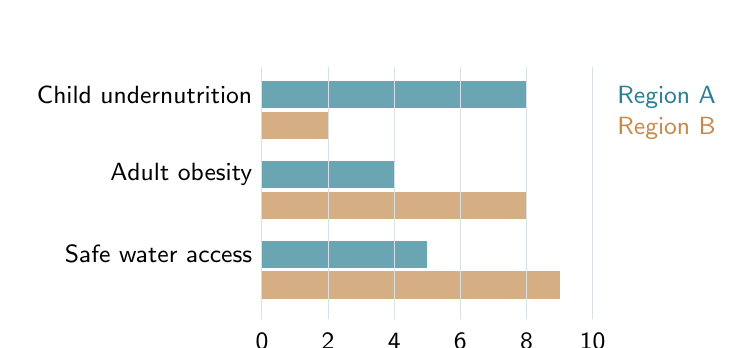
\begin{tikzpicture}[x=0.42cm,y=0.78cm, every node/.style={font=\sffamily\small}]
  \node[anchor=east] at (0,3) {Child undernutrition};
  \draw[fill=AccentTeal!70, draw=none] (0,2.78) rectangle (8,3.22);
  \draw[fill=AccentGold!70, draw=none] (0,2.28) rectangle (2,2.72);
  \node[anchor=east] at (0,1.7) {Adult obesity};
  \draw[fill=AccentTeal!70, draw=none] (0,1.48) rectangle (4,1.92);
  \draw[fill=AccentGold!70, draw=none] (0,0.98) rectangle (8,1.42);
  \node[anchor=east] at (0,0.4) {Safe water access};
  \draw[fill=AccentTeal!70, draw=none] (0,0.18) rectangle (5,0.62);
  \draw[fill=AccentGold!70, draw=none] (0,-0.32) rectangle (9,0.12);
  \foreach \x in {0,2,4,6,8,10} {
    \draw[RuleGray] (\x,-0.65) -- (\x,3.45);
    \node[anchor=north] at (\x,-0.72) {\x};
  }
  \node[anchor=west, color=AccentTeal] at (10.45,2.95) {Region A};
  \node[anchor=west, color=AccentGold] at (10.45,2.45) {Region B};
\end{tikzpicture}
\end{center}

\subsection{Questions}

Answer all questions under timed conditions.

\begin{enumerate}
  \item \exam{State} two contrasts between Region A and Region B shown in
  Source A. \hfill \textbf{2 points}
  \item \exam{Describe} two ways food and health indicators can show inequality.
  \hfill \textbf{4 points}
  \item \exam{Explain} two reasons why food systems can influence health
  outcomes. \hfill \textbf{4 points}
  \item \exam{Using Brazil and Nestle, or the named Food and health case study
  you have studied}, \exam{examine} the role of stakeholders in improving or
  worsening food security and health. \hfill \textbf{10 points}
\end{enumerate}

\subsection{Timing Guide}

\begin{tabularx}{\textwidth}{L{0.2\textwidth}Y}
\toprule
\textbf{Question} & \textbf{Time limit and writing goal} \\
\midrule
Question 1 & 3 minutes. Two clear contrasts using Source A evidence. \\
Question 2 & 5 minutes. Two indicator-based descriptions; mention what each
indicator shows and what it may hide. \\
Question 3 & 7 minutes. Two concise causal chains linking food-system factors
to health outcomes. \\
Question 4 & 15 minutes. Named case study, stakeholder roles, benefits, costs,
and a balanced judgment. This trains the 10-mark extended-answer habit. \\
\bottomrule
\end{tabularx}

\subsection{Brazil And Nestle Answer Frame For Question 4}

For Brazil and Nestle, a strong answer can argue that TNCs are important
stakeholders because they influence food availability, supply chains, marketing,
employment, and consumer diets. A precise hook is \term{Nestle Ate Voce}, the
company's Brazilian door-to-door microdistribution model, and \term{Nestle Ate
Voce a Bordo}, a floating supermarket initiative launched in 2010 to reach
communities along the Amazon. Benefits may include investment, jobs,
micro-distributor income, distribution networks, and wider product access. The
evaluation is that TNC activity can also encourage processed-food consumption,
shape diets through advertising, and shift power away from small producers or
public-health priorities. A balanced conclusion should judge whether corporate
involvement mainly improves access and livelihoods or deepens diet-related
health risks and unequal power.

\section{20-Minute Mark And Error Log}

\subsection{Self-Mark Guide}

\rowcolors{2}{TableStripe}{white}
\begin{tabularx}{\textwidth}{L{0.13\textwidth}Y Y}
\toprule
\textbf{Question} & \textbf{Credit-worthy content} & \textbf{Common mistakes} \\
\midrule
1 & Two direct contrasts from Source A, such as high child undernutrition in
Region A versus low in Region B, or processed-food concern in Region B versus
limited food access in Region A & Explaining before stating, or adding claims
not shown in the source \\
2 & Clear descriptions of inequality using indicators such as safe water,
healthcare access, undernutrition, obesity, and disease risk. Strong answers
state what the indicator shows and what it hides & Listing indicators without
saying how they show inequality \\
3 & Two causal chains. Examples: weak storage $\rightarrow$ spoilage
$\rightarrow$ lower food availability; processed-food marketing $\rightarrow$
high sugar/salt/fat diets $\rightarrow$ obesity or NCD risk; unsafe water
$\rightarrow$ contamination $\rightarrow$ infectious disease & Describing a food
system without linking it to health outcomes \\
4 & Named case study, stakeholder roles, benefits, costs, and judgment. For
Brazil and Nestle, discuss TNC investment and distribution, such as Nestle Ate
Voce, alongside processed foods, marketing, consumer health, and power. Include
at least one other stakeholder such as government, consumers, farmers, or
public-health groups &
No named example, no stakeholder contrast, no evaluation, or treating the TNC as
only positive or only negative \\
\bottomrule
\end{tabularx}
\rowcolors{2}{}{}

\subsection{Command-Term Checks}

\begin{itemize}
  \item \exam{State}: give a short answer. Do not explain unless asked.
  \item \exam{Describe}: say what the source or indicator shows.
  \item \exam{Explain}: give a reason and show the causal chain.
  \item \exam{Examine}: look at more than one side and reach a supported
  judgment.
\end{itemize}

\subsection{Error Log Categories}

Use the workbook to write the full error log. Classify every error into one of
these categories:

\rowcolors{2}{TableStripe}{white}
\begin{tabularx}{\textwidth}{L{0.22\textwidth}Y Y}
\toprule
\textbf{Category} & \textbf{What it means} & \textbf{Fix before the next session} \\
\midrule
Command term & You answered the wrong task, such as explaining when asked to
describe & Rewrite the first sentence using the exact command term \\
Source use & You ignored Source A or made unsupported claims & Add two source
phrases or contrasts \\
Process chain & You listed factors but did not show how they affect health &
Add \term{because}, \term{therefore}, and one health outcome \\
Case evidence & Your named example was too vague & Add place, actor, product or
policy, impact, and time frame if known \\
Evaluation & You did not judge stakeholders, scale, winners, losers, or
limitations & Add \term{however}, \term{whereas}, or \term{this is limited
because} \\
\bottomrule
\end{tabularx}
\rowcolors{2}{}{}

\section{10-Minute Case-Study Drill}

Use this final block only for case-study names and one evaluative point for
each. The keyword table belongs to the recall block.

\begin{tabularx}{\textwidth}{L{0.23\textwidth}Y Y}
\toprule
\textbf{Case-study anchor} & \textbf{Minimum recall} & \textbf{Evaluative point} \\
\midrule
Brazil and Nestle & Place, actor, product or food-system role, and one health
or food-security impact & TNCs can improve access and investment while also
raising concern about processed-food diets, marketing power, and inequality \\
Studied disease case, or skip if not covered & Disease, place, transmission
route, vulnerable group, and response & A response may reduce spread but be
limited by poverty, healthcare access, trust, or infrastructure \\
Studied food-security case & Place, cause of food insecurity, affected group,
and response & Aid or policy may treat short-term hunger while leaving
structural causes unresolved \\
Future food or health example & Strategy, stakeholder, intended benefit, and
cost & Sustainability responses need evaluation by cost, access, scale, and
who benefits \\
\bottomrule
\end{tabularx}

\section{End-Of-Day Output}

You are finished with April 26 if you have:

\begin{itemize}
  \item redrawn the four-cluster Food and health map from memory
  \item explained one food-system chain using process language
  \item explained at least two factors affecting disease spread
  \item written one timed structured-question response in 30 minutes
  \item marked the answer and identified at least three specific errors
  \item drilled case-study names and one evaluative point for each
  \item updated your mastery rating for Food and health
\end{itemize}

\boxnote{SoftGreen}{Carry forward.}{On Tuesday 2026-04-28, the plan returns to
Food and health with Resources. Bring forward the weakest food-system,
disease-spread, or stakeholder-evaluation detail from today's error log.}

\end{document}
